\documentclass[12pt]{article}
\usepackage[utf8]{inputenc}
\usepackage[greek,english]{babel}
\usepackage{alphabeta}
\usepackage{fancyhdr}
\usepackage{listings}
\usepackage{mathtools}
\usepackage{xcolor}
\usepackage{float}
\usepackage{siunitx}
\usepackage[margin=0.5in]{geometry}
\usepackage[backend=bibtex]{biblatex}

\lstset {
        basicstyle=\ttfamily,
        columns=fullflexible,
        breaklines=true,
        keepspaces=true,
	showstringspaces=false
}

\title{Εργαστήριο Ασφάλειας στην Τεχνολογία της Πληροφορίας -- Εργασία 1}
\author{Χρήστος Μαργιώλης -- 19390133}
\date{Απρίλιος 2023}

\begin{document}

\begin{titlepage}
        \maketitle
        \begin{figure}[t!]
        \begin{center}
        
\includegraphics[scale=0.3]{./res/uniwalogo.png} \\
        \Large
        \textbf{Πανεπιστήμιο Δυτικής Αττικής} \\
        \large
        Τμήμα Μηχανικών Πληροφορικής και Ηλεκτρονικών Υπολογιστών
        \end{center}
        \end{figure}
\end{titlepage}

\renewcommand{\contentsname}{Περιεχόμενα}
\tableofcontents
\pagebreak

\section{Δραστηριότητα 1: Ανάπτυξη και δοκιμή του shellcode}

Αρχικά απενεργοποιούμε το ASLR: \\

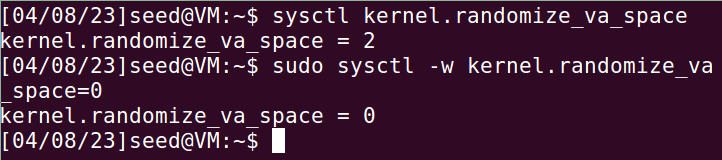
\includegraphics[width=\textwidth]{res/aslr.png} \\

Γράφουμε το πρόγραμμα \lstinline{shellcode.c}:

\lstinputlisting[language=c]{../src/shellcode.c}

Κάνουμε compile και το τρέχουμε: \\

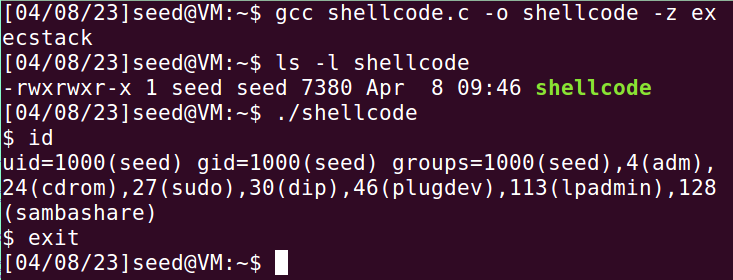
\includegraphics[width=\textwidth]{res/shellcode.png} \\

Μετατρέπουμε το πρόγραμμα σε setuid: \\

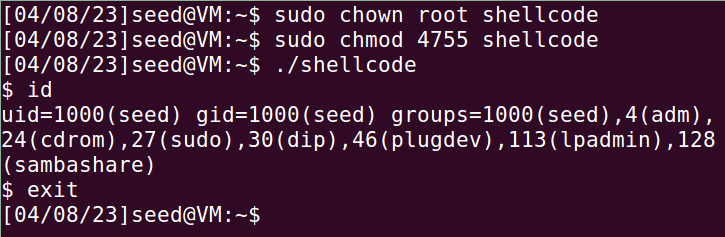
\includegraphics[width=\textwidth]{res/chownshellcode.png} \\

Παράκαμψη αντιμέτρου \lstinline{/bin/sh} δημιουργώντας symbolic link με το
\lstinline{/bin/zsh} και επανεκτέλεση του προγράμματος: \\

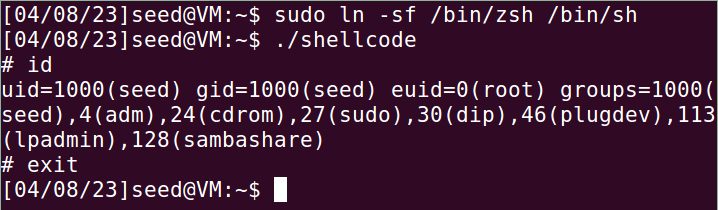
\includegraphics[width=\textwidth]{res/zshshellcode.png} \\

\section{Δραστηριότητα 2: Ανάπτυξη του ευπαθούς προγράμματος}

\lstinputlisting[language=c]{../src/stack.c}

Κάνουμε compile και το τρέχουμε: \\

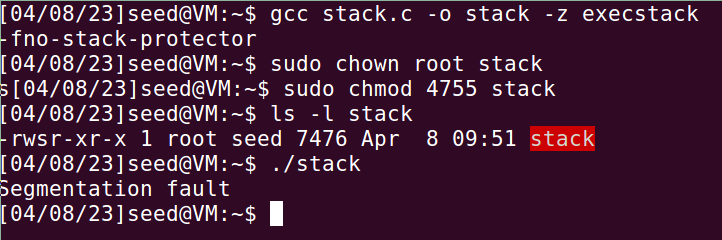
\includegraphics[width=\textwidth]{res/stack.png} \\

\section{Δραστηριότητα 3: Δημιουργία του αρχείου εισόδου (badfile)}

\lstinputlisting[language=c]{../src/exploit.c}

Κάνουμε compile και τρέχουμε το πρόγραμμα ώστε να παραχθεί το αρχείο εισόδου: \\

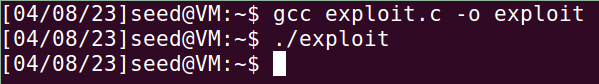
\includegraphics[width=\textwidth]{res/exploit.png} \\

Αναλύουμε τα περιεχόμενα του badfile μέσω του προγράμματος hexdump: \\

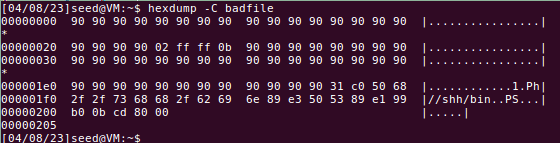
\includegraphics[width=\textwidth]{res/hexdump.png} \\

\section{Δραστηριότητα 4: Εύρεση της διεύθυνσης του shellcode μέσα στο badfile}

Κάνουμε compile το πρόγραμμα δίνοντας την επιλογή \lstinline{-g} ώστε να
παραχθει debug δεδομένα τα οποία θα χρησιμοποιηθούν από τον GDB: \\

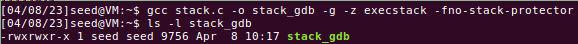
\includegraphics[width=\textwidth]{res/stack_gdb.png} \\

Βάζουμε breakpoint στην συνάρτηση \lstinline{bof()} και τρέχουμε το πρόγραμμα στον
GDB: \\

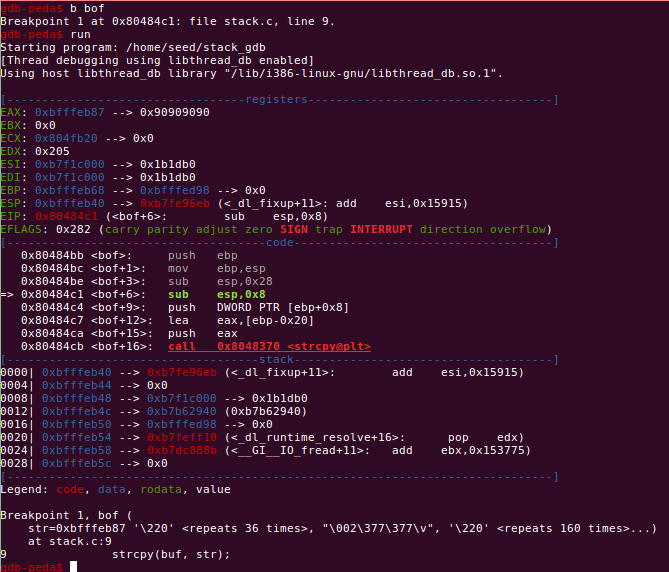
\includegraphics[width=\textwidth]{res/gdb1.png} \\

Τυπώνουμε τις διευθύνσεις του buffer, καθώς και του καταχωρητή \lstinline{ebp}
και τέλος υπολογίζουμε την απόστασή τους: \\

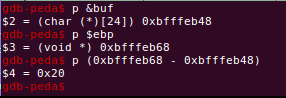
\includegraphics[width=\textwidth]{res/gdb2.png} \\

\section{Δραστηριότητα 5: Προετοιμασία του αρχείου εισόδου}

Τροποποιούμε τον κώδικα του \lstinline{exploit.c} ώστε να δείχνει στην σωστή
διεύθυνση μνήμης (το offset \lstinline{0x60} προέκυψε μετά από δοκιμές):

\begin{lstlisting}[language=C]
	*((long *)(buf + 0x24)) = 0xbfffeb48 + 0x60;
\end{lstlisting}

Μεταγλωττίζουμε και ελέγχουμε το νέο badfile: \\

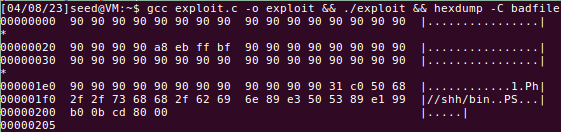
\includegraphics[width=\textwidth]{res/offset.png} \\

\section{Δραστηριότητα 6: Εκτέλεση της επίθεσης}

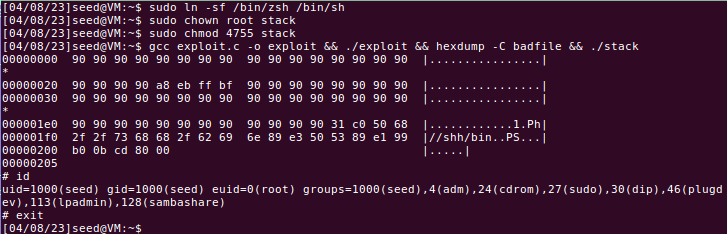
\includegraphics[width=\textwidth]{res/attack.png} \\

\end{document}
